%----------------------------------------------------------------------------------------
%
% A LaTeX-template 
%
%----------------------------------------------------------------------------------------

% Settings and document configuration

\documentclass[a4paper,12pt]{article} 
\usepackage[T1]{fontenc} 
\usepackage{times} 
\usepackage[swedish,english]{babel} 
\usepackage[utf8]{inputenc} 
\usepackage{dtk-logos} 
\usepackage{wallpaper} 
\usepackage[absolute]{textpos} 
\usepackage[top=2cm, bottom=2.5cm, left=3cm, right=3cm]{geometry} 
\usepackage[parfill]{parskip} 
\usepackage{csquotes} 
\usepackage{float} 
\usepackage{lipsum} % Used for dummy text. Can be removed.
\usepackage{pdflscape} % Para documentos en formato PDF
\usepackage{listings}
\usepackage{hyperref}


% Fontsizes for section headings.
\usepackage{sectsty} 
\sectionfont{\fontsize{14}{15}\selectfont}
\subsectionfont{\fontsize{12}{15}\selectfont}
\subsubsectionfont{\fontsize{12}{15}\selectfont}

%----------------------------------------------------------------------------------------
%	This part is used for the text box on the title page
%----------------------------------------------------------------------------------------
\newsavebox{\mybox}
\newlength{\mydepth}
\newlength{\myheight}

\newenvironment{sidebar}%
{\begin{lrbox}{\mybox}\begin{minipage}{\textwidth}}%
{\end{minipage}\end{lrbox}%
 \settodepth{\mydepth}{\usebox{\mybox}}%
 \settoheight{\myheight}{\usebox{\mybox}}%
 \addtolength{\myheight}{\mydepth}%
 \noindent\makebox[0pt]{\hspace{-20pt}\rule[-\mydepth]{1pt}{\myheight}}%
 \usebox{\mybox}}

%----------------------------------------------------------------------------------------
%	Title
%----------------------------------------------------------------------------------------
\newcommand\BackgroundPic{
    \put(-2,-3){
    
\includegraphics[keepaspectratio,scale=1.5]{img/su_olivier1.png} % Background image
    }
}
\newcommand\BackgroundPicLogo{
    \put(15,710){
    
\includegraphics[keepaspectratio,scale=0.2]{img/logo.png} % LNU logo
    }
}

\title{
\vspace{-8cm}
\begin{sidebar}
    \vspace{10cm}
    \normalfont \normalsize
    \huge Reporte\\ % Main title
    \vspace{-1.3cm}
\end{sidebar}
\vspace{3cm}
\begin{flushleft}
    \huge My Red % Subtitle
\end{flushleft}
\null
\vfill
\begin{textblock}{5}(10,13)
\begin{flushright}
\begin{minipage}{\textwidth}
\begin{flushleft} \large
\emph{Author:} Eugenio Cortes Carlos \\  % Author
\date{08/06/2021}
\end{flushleft}
\end{minipage}
\end{flushright}
\end{textblock}
}

\date{} % Empty date command. Use \today inside for today's date.
\author{} % Normally one would use this to define authors. However in this case the title command takes care of everything, so we leave the field empty to get rid of warnings. 

\begin{document}

\pagenumbering{gobble} % Turn off page numbering
\newgeometry{left=5cm}
\AddToShipoutPicture*{\BackgroundPic} % Adds the background image to the title page
\AddToShipoutPicture*{\BackgroundPicLogo} % Adds the logo to the title page
\maketitle % Prints the title
\restoregeometry
\clearpage

\pagenumbering{roman} % Roman page numbering for abstract page

%\selectlanguage{english}
%\begin{abstract}
%\noindent English abstract.
%\end{abstract}

\newpage

\pagenumbering{gobble} % Turn off page numbering
\tableofcontents

\newpage
\pagenumbering{arabic} % Turn on page numbering

% Some example sections with dummy text
\section{Introducción}
Hoy en día el internet es una herramienta fundamental que forma parte de nuestra vida, por ende surge la necesidad de contar con herramientas especializadas que permitan administrar de manera efectiva y organizada a los usuarios de diversos pueblos. Con este objetivo en mente, se desarrolló la aplicacion : "MyRed".

El objetivo principal de este proyecto es proporcionar una solución integral para la gestión de usuarios, permitiendo registrar y organizar de manera eficiente a cada individuo según su ubicación geográfica en diferentes pueblos. Esto brinda una visión clara y eficiente de los usuarios, lo cúal facilita la administración de sus datos y mantenimiento del servicio. 

Para lograr este objetivo, se ha adoptado la metodología SCRUM en el proceso de desarrollo. SCRUM ha permitido desarrollar el proyecto de manera iterativa e incremental, dividiéndolo en sprints para obtener entregas rápidas y ajustar el desarrollo de acuerdo a las necesidades del cliente. Esta metodología ha demostrado ser altamente eficiente y ha permitido mantener un enfoque constante en la calidad del producto final.

En cuanto a las herramientas y tecnologías utilizadas, se ha empleado un enfoque basado en web para el desarrollo del Administrador de Usuarios. El lenguaje de programación principal utilizado es HTML (HyperText Markup Language), que permite estructurar y dar forma a las páginas web. Para el diseño y la presentación visual, tambien se ha utilizado CSS (Cascading Style Sheets), el cual brinda la capacidad de personalizar y estilizar la apariencia de las páginas.

Además, se  ha hecho uso de JavaScript el cual tuvo la función de otorgar al sistema interactividad y dinamismo, permitiendo una usabilidad más sencilla y eficiente. Para el almacenamiento y gestión de los datos de los usuarios, hemos empleado una base de datos en MySQL, que se integra con el sistema a través de XAMPP y Php, estos dos en conjunto permitieron el registro dentro de la base de datos, cubriendo los requerimientos establecidos por el usuario.

% Nueva página para la sección "Planificación"

\newpage
\begin{landscape}
  \begin{figure}
  \section{Planificación}
    \centering
    \includegraphics[width=1.8\textwidth]{Latex_Template/img/DiagramaGantt3.png}
    \caption{Diagrama de Gantt}
    \label{fig:image}
  \end{figure}
\end{landscape}

% Nueva página para la sección "Diseño"
\newpage
\section{Diseño}
En esta sección del reporte, se detallarán los aspectos relacionados con el diseño del proyecto, incluyendo los requisitos funcionales y no funcionales, el modelo de base de datos, los casos de uso y las historias de usuario.

\subsection{\textbf{Requisitos Funcionales.}} \\
Los requisitos funcionales describen las funcionalidades específicas que debe cumplir el sistema. A continuación, se presentan los requisitos cubiertos al desarrollar el proyecto de MyRed:

\textbf{Registro de usuarios:} Permitir el registro de nuevos usuarios en el sistema, proporcionando información como nombre, apellido, población, monto a pagar, fecha de inicio, nombre del modem, nombre de la antena y contraseñas implementadas. 

\textbf{Gestión de usuarios:} Permitir la visualización, edición y eliminación de los datos de los usuarios registrados.

\textbf{Generación de reportes:} Proporcionar la capacidad de generar informes y reportes personalizados sobre la información de los usuarios, como el estado de pago y el rendimiento de la red. 
\\

\subsection{\textbf{Requisitos No Funcionales}}\\
Los requisitos no funcionales se refieren a las características no específicas de funcionalidad del sistema, pero que son igualmente importantes para su diseño y desarrollo. Los requisitos empleado en nuestro proyecto son: 

\textbf{Usabilidad:} El sistema debe ser intuitivo y fácil de usar para los usuarios finales, con una interfaz de usuario clara y bien organizada.

\textbf{Rendimiento:} El sistema debe ser capaz de manejar grandes volúmenes de usuarios y datos de manera eficiente, con tiempos de respuesta rápidos y sin problemas de rendimiento.

\textbf{Seguridad:} El sistema debe garantizar la seguridad de los datos de los usuarios, implementando medidas de protección, como cifrado de contraseñas.
\\

\subsection{\textbf{Modelo de Base de Datos.}}\\
El modelo de base de datos describe la estructura y las relaciones de las entidades y tablas que se utilizarán para almacenar la información del sistema. Para el caso de este proyecto (MyRed), incluye las tablas: Usuario, contratos, DetallesRed, Pueblos. Las cuales todas están relacionadas con la tabla Contratos, con una relacion 1:N (uno a muchos), de esta forma evitamos la redundancia en los datos.

\subsection{\textbf{Casos de Uso.}}\\
Los casos de uso representan las interacciones entre los usuarios y el sistema. Para la elaboración de este proyecto los casos de uso que se cubrieron fueron: Inicio de sesión, Menu de asignación, Menu principal y reporte mensual. Cuyos diagramas se encuentran anexados al final del presente documento. 

\subsection{\textbf{Historias de Usuario}}\\
Las historias de usuario son breves descripciones de funcionalidades específicas del sistema, escritas desde la perspectiva del usuario. Estas describen qué desea lograr el usuario y por qué. Las historias de usuario para este proyecto son las siguientes. 
\begin{enumerate}
    \item Como usuario, quiero iniciar sesión en la aplicación MyRed para acceder a sus funciones y administrar mis pueblos y clientes\\
    \item Como usuario, quiero asignar nuevos clientes en la aplicación para mantener mi base de datos actualizada.\\
    \item Como usuario, quiero ver la lista de clientes en un pueblo específico junto con su información para llevar un control de mi red.\\
    \item  Como usuario, quiero buscar clientes, módulos, puntos de acceso o servicios en la aplicación para poder encontrar rápidamente la información que necesito.\\
    \item Como usuario, quiero agregar y eliminar clientes en la aplicación MyRed para mantener mi base de datos de clientes precisa y actualizada.\\
\end{enumerate}



% Nueva página para la sección "Codificación"
\newpage
\section{Codificación}
En esta etapa, se muestra el codigo completo que se empleo para la creacion del presente proyecto. Dicho codigo fué realizado en los entornos de html, css, JavaScript, Php: \\

\subsection{Código de la aplicación web}
El siguiente Link redirige a GitHub Gist, en donde se encuentra el codigo del proyecto completo

\href{https://gist.github.com/EugenioCCA/d96bc43e9fea3f9beb9c5ff4ac806b58}{Código del proyecto MyRed}

\subsection{Diagrama Entidad Relación}
\begin{figure}[ht]
  \centering
  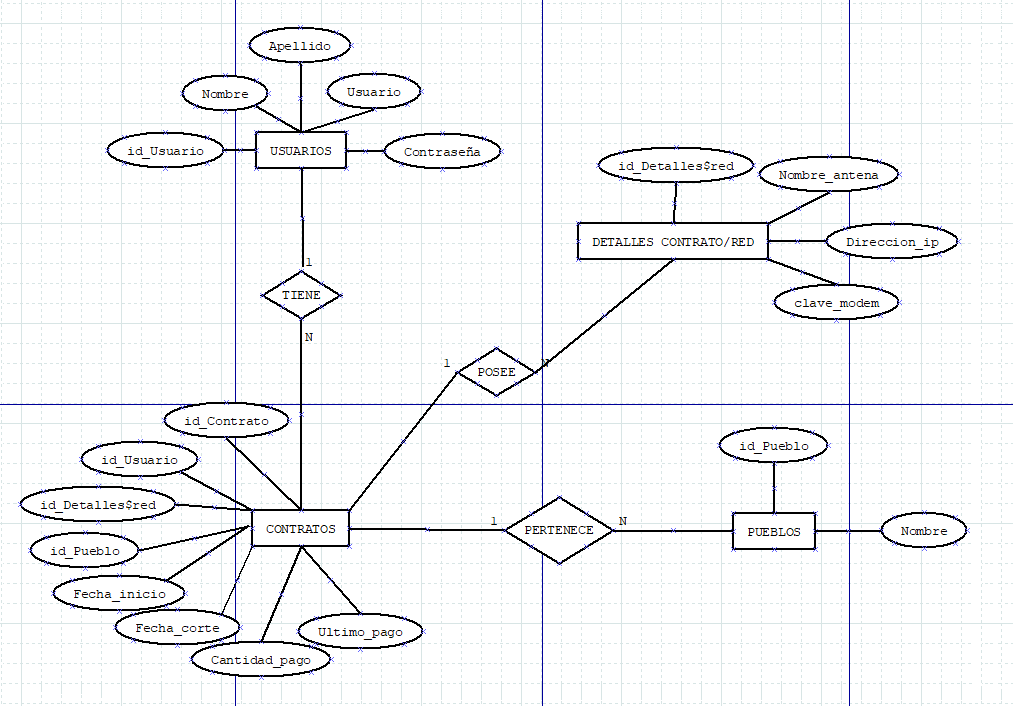
\includegraphics[width=.5\textwidth]{Latex_Template/img/diagramaER.png}
    \caption{Diagrama Entidad Relación}
    \label{fig:image}
\end{figure}

\subsection{Diagrama Relacional}
\begin{figure}[ht]
  \centering
  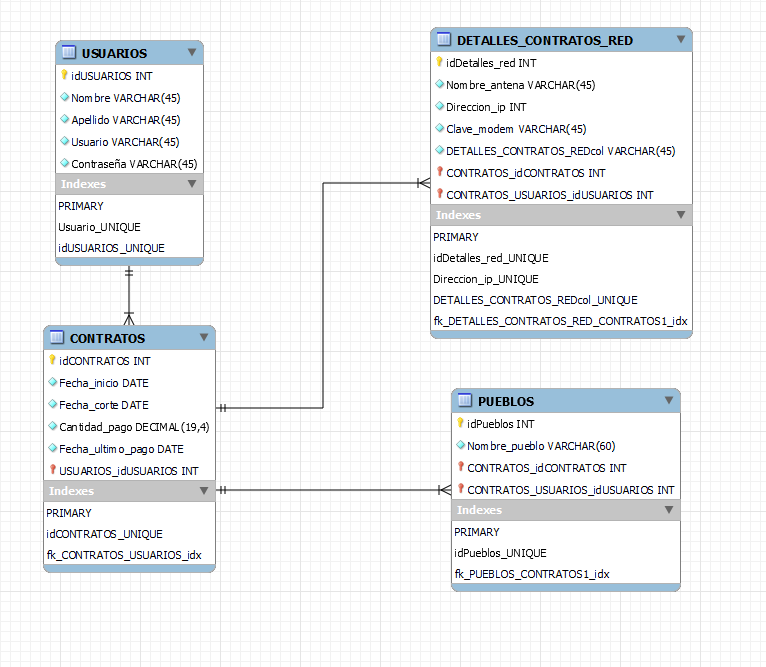
\includegraphics[width=.6\textwidth]{Latex_Template/img/diagramaRelacional.png}
    \caption{Diagrama Relacional}
    \label{fig:image}
\end{figure}

\subsection{Diagrama fisico}
\begin{lstlisting}[language=Sql, basicstyle=\footnotesize\ttfamily, numbers=left]
\begin{verbatim}
CREATE DATABASE MyRedDB;

USE MyRedDB;

CREATE TABLE USUARIOS (
    idUsuario INT NOT NULL PRIMARY KEY,
    Nombre VARCHAR(45) NOT NULL,
    Apellido VARCHAR(45) NOT NULL,
    Usuario VARCHAR(45) NOT NULL UNIQUE,
    Contraseña VARCHAR(45) NOT NULL UNIQUE
);

Use MyRedDB; 
CREATE TABLE PUEBLOS (
    idPueblo INT NOT NULL PRIMARY KEY,
    Nombre_pueblo VARCHAR(60) NOT NULL
);

Use MyRedDB; 
CREATE TABLE CONTRATOS (
    idContrato INT NOT NULL PRIMARY KEY,
    Fecha_inicio DATE NOT NULL,
    Fecha_corte DATE NOT NULL,
    Cantidad_pago DECIMAL(19,4) NOT NULL,
    Fecha_ultimo_pago DATE NOT NULL,
    idUsuario INT,
    idPueblo INT,
    idDatosRed INT, 
    FOREIGN KEY (idUsuario) REFERENCES USUARIOS(idUsuario),
    FOREIGN KEY (idPueblo) REFERENCES PUEBLOS(idPueblo),
    FOREIGN KEY (idDatosRed) REFERENCES DETALLES_CONTRATOS_RED(idDetalles)
);


Use MyRedDB; 
CREATE TABLE DETALLES_CONTRATOS_RED (
    idDetalles INT NOT NULL PRIMARY KEY,
    Nombre_antena VARCHAR(45) NOT NULL,
    Direccion_ip VARCHAR(25) NOT NULL UNIQUE,
    Clave_modem VARCHAR(45) NOT NULL,
    idContrato INT,
    FOREIGN KEY (idContrato) REFERENCES CONTRATOS(idContrato)
);



\end{verbatim}
\end{lstlisting}

% Nueva página para la sección "Pruebas"
\newpage
\section{Pruebas}
La sección de Pruebas es fundamental en el desarrollo de cualquier proyecto, ya que permite verificar y validar el funcionamiento correcto del sistema. En esta etapa, se llevan a cabo una serie de pruebas para asegurarse de que el software cumple con los requisitos establecidos y se comporta de acuerdo con las expectativas.

El objetivo principal de esta sección es presentar las diferentes pruebas realizadas, tanto funcionales como no funcionales, y describir los resultados obtenidos.

\subsection{Prueba1. Login}
Datos de entrada: Usuario y contraseña
Resultado esperado: Acceder al menú principal\\

Acciones: Se comprueba en la base de datos que el usuario y contraseña existan para permitir el acceso.\\

Resultados
Resultado obtenido: La conexión funciona de forma correcta
Resultado esperado: Conexión correcta
Resultado de la prueba: Prueba exitosa\\



\begin{figure}[ht]
  \centering
  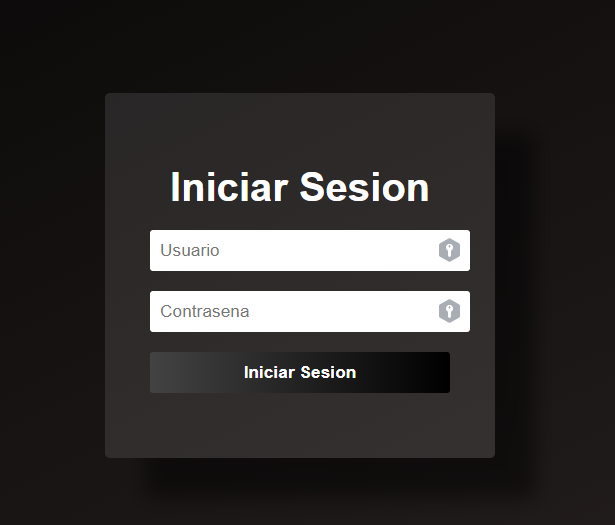
\includegraphics[width=.9\textwidth]{Latex_Template/img/inicio.png}
    \centering\caption{Inicio de sesión}
    \label{fig:image}
\end{figure}

    



\subsection{Prueba2. Funcionalidad de la pagina}
Datos de entrada: Cambiar entre las distintas opciones que tiene el menú. 
Resultado esperado: Que no haya ningun errror al cargar las diferentes pantallas\\

Acciones: se hace uso del codigo de JavaScript ya que es el encargado de la funcionalidad e interacción\\

Resultados
Resultado obtenido: Todas las opciones mostraron la información correcta. 
Resultado esperado: Que no hubiera errores al mostrar información. 
Resultado de la prueba: Prueba exitosa\\

\begin{figure}[ht]
  \centering
  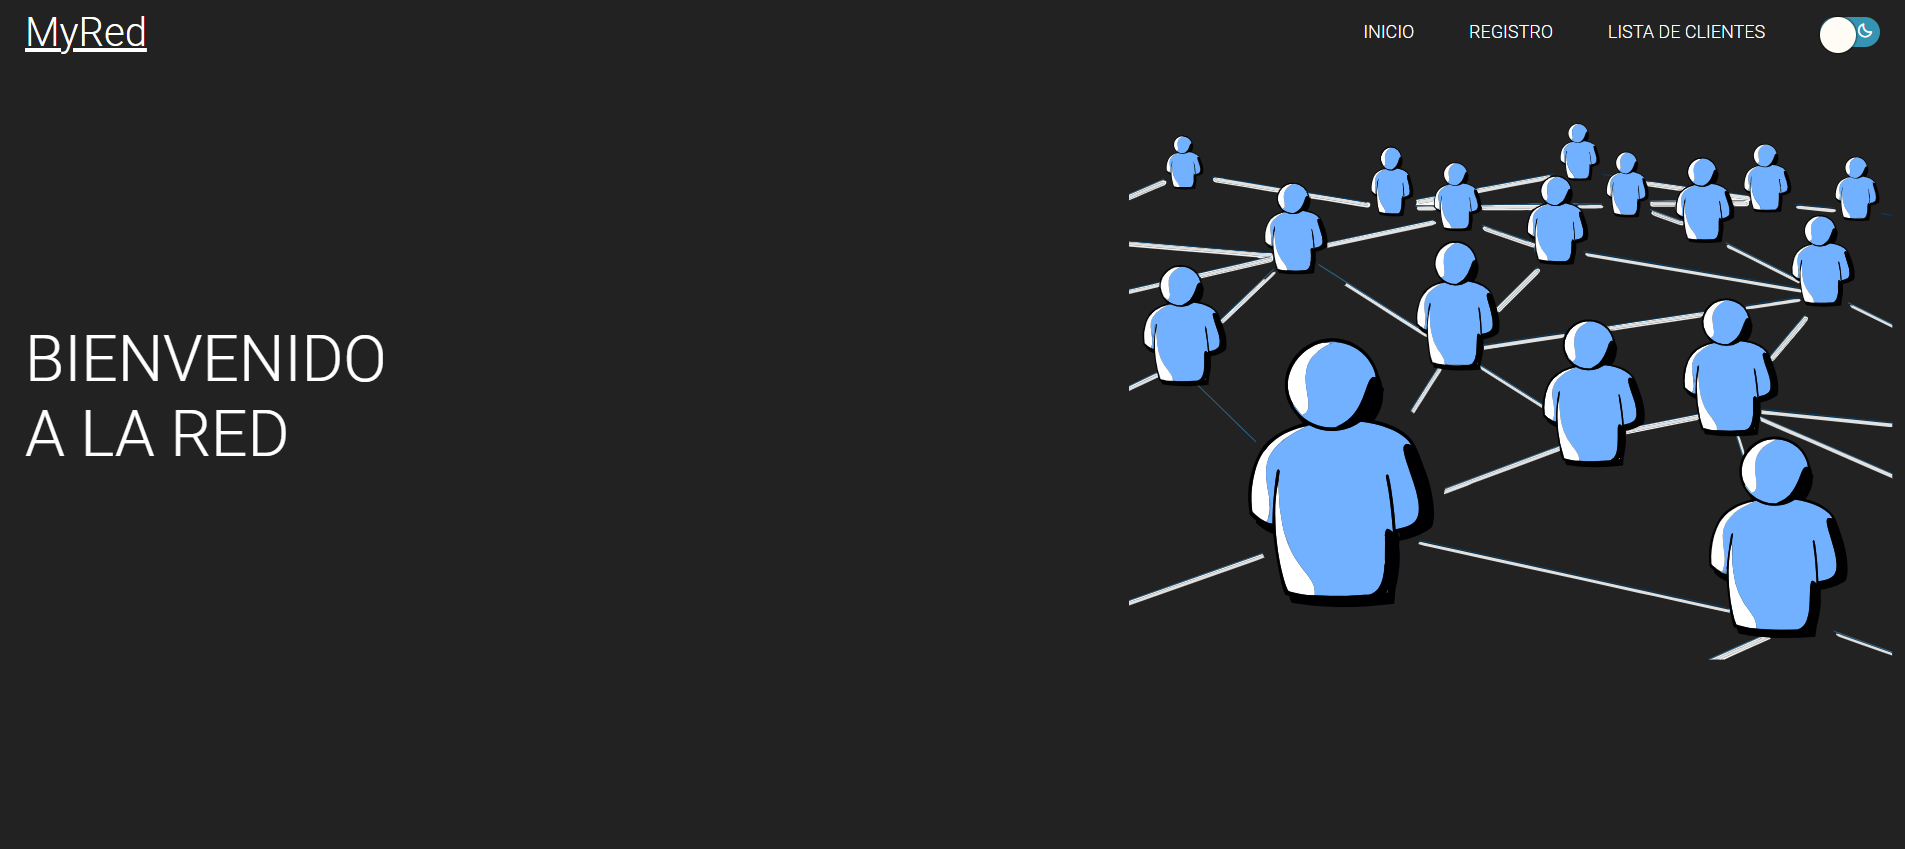
\includegraphics[width=.9\textwidth]{Latex_Template/img/pantallaInicio.png}
    \caption{Pantalla de inicio}
    \label{fig:image}
\end{figure}


\subsection{Prueba3. Registro de clientes}
Datos de entrada: Rellenar el formulario en la opción de registro. 
Resultado esperado: Los datos ingresados aparezcan en la base de datos\\

Acciones: Se hace uso de Php para establecer la conexion y hacer el INSERT INTO a la base de datos \\

Resultados
Resultado obtenido: Los datos se ingresaron a la DB(Base de Datos) de forma correcta.
Resultado esperado: Que no hubiera problemas al hacer la inserción de los datos en la DB. 
Resultado de la prueba: Prueba exitosa\\

\begin{figure}[ht]
  \centering
  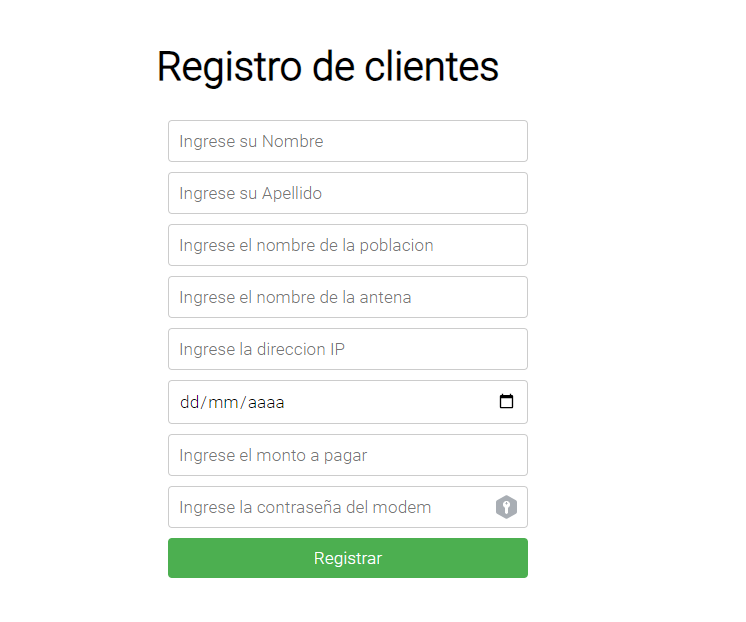
\includegraphics[width=.9\textwidth]{Latex_Template/img/resgistro.png}
    \caption{Registro de clientes}
    \label{fig:image}
\end{figure}

\subsection{Prueba4. Mostrar clientes}
Datos de entrada: Seleccionar la opcion "Lista de clientes" en el panel de opciones. 
Resultado esperado: Se muestren todos los clientes registrados en la Base de Datos de forma ordenada y sin detalles.\\

Acciones: Se hace uso de Php para establecer la conexion con la DB y hacer el SELECT FROM a las tablas correspondientes. \\

Resultados
Resultado obtenido: Los clientes se mostraron de forma correcta, con todos sus datos ordenados. 
Resultado esperado: Que no hubiera errores al presentar la información de los usuarios. 
Resultado de la prueba: Prueba exitosa\\

\begin{figure}[ht]
  \centering
  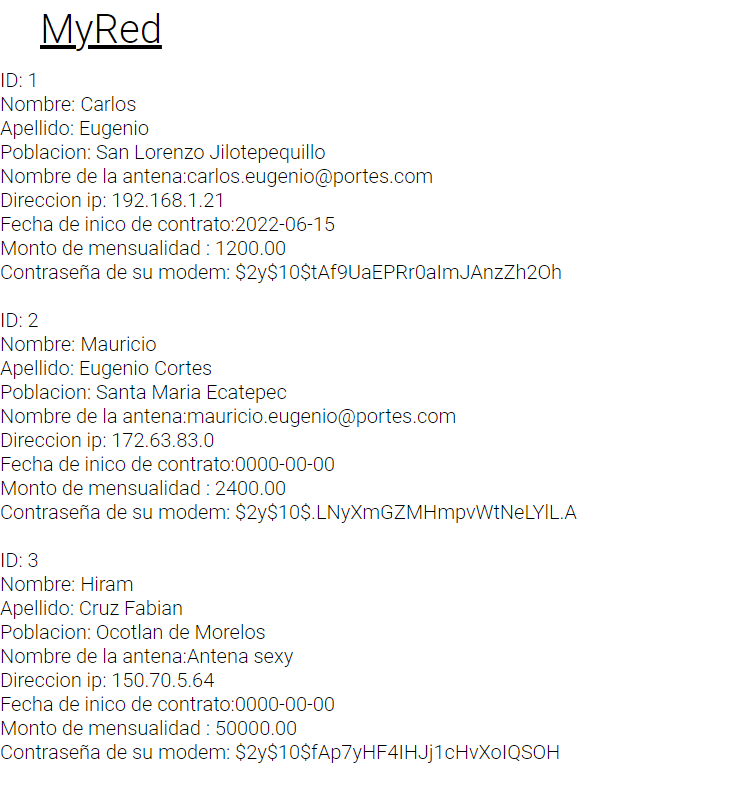
\includegraphics[width=.9\textwidth]{Latex_Template/img/clientes.png}
    \caption{Vista de clientes registrados}
    \label{fig:image}
\end{figure}

% Nueva página para la sección "Resultados"
\newpage
\newpage
\section{Resultados}
En esta última sección del proyecto, se mostrará evidencia de todo lo realizado a lo largo del proyecto. 
\begin{figure}[ht]
  \centering
  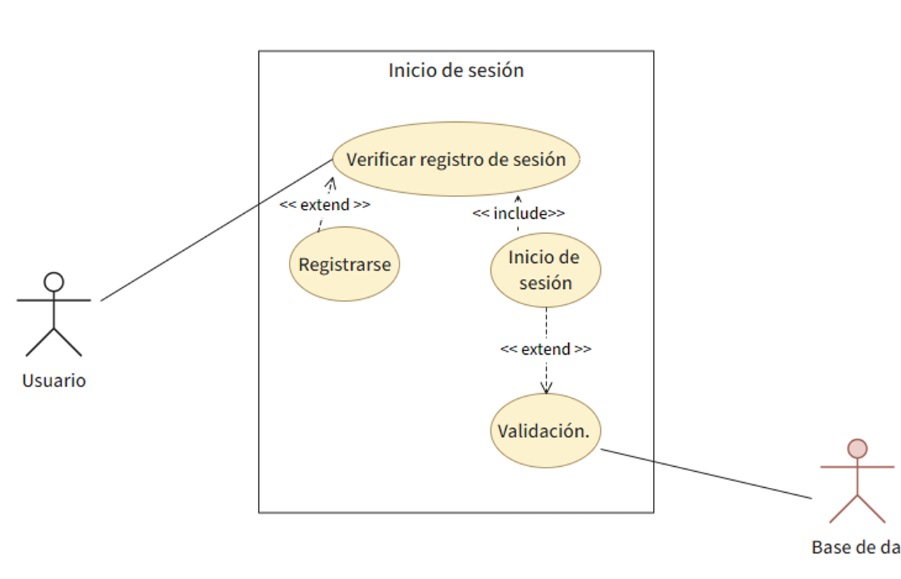
\includegraphics[width=.9\textwidth]{Latex_Template/img/casosUso1.png}
    \caption{Caso Uso. login}
    \label{fig:image}
\end{figure}\\

\begin{figure}[ht]
  \centering
  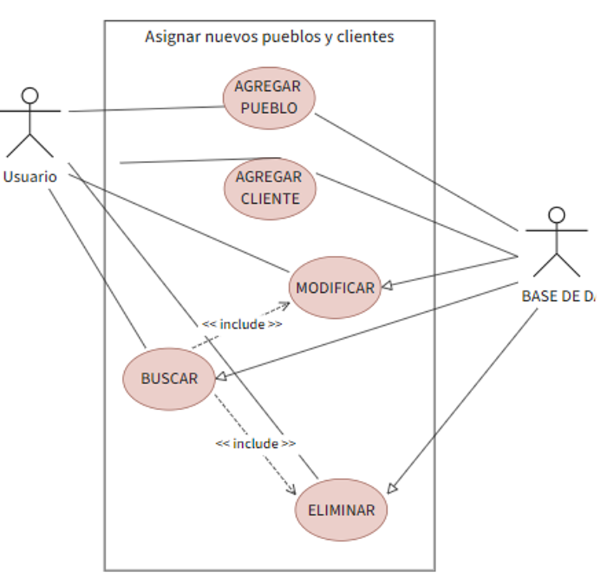
\includegraphics[width=.9\textwidth]{Latex_Template/img/casoUso2.png}
    \caption{Caso Uso. registro}
    \label{fig:image}
\end{figure}\\

\begin{figure}[ht]
  \centering
  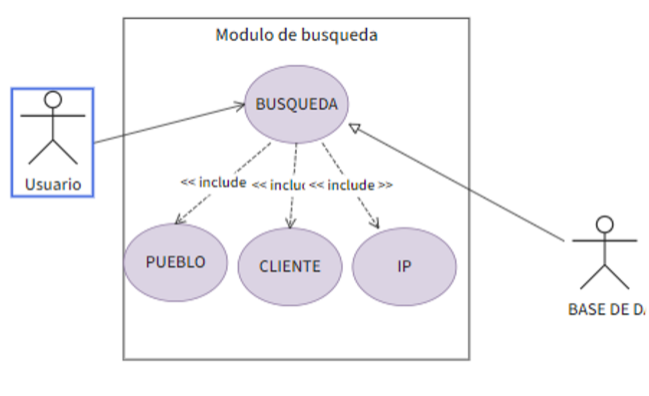
\includegraphics[width=.9\textwidth]{Latex_Template/img/casoUso3.png}
    \caption{Caso Uso. Busqueda}
    \label{fig:image}
\end{figure}\\


\begin{figure}[ht]
  \centering
  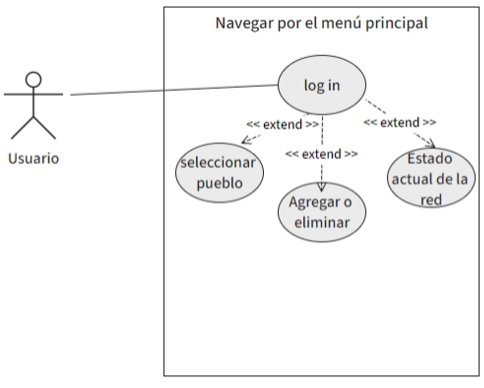
\includegraphics[width=.9\textwidth]{Latex_Template/img/casoUso4.png}
    \caption{Caso Uso. Navegar en menú }
    \label{fig:image}
\end{figure}\\


\end{document}
